% Euclidean Handout Number fourteen
\documentclass{tufte-handout}

%\geometry{showframe}% for debugging purposes -- displays the margins

%%%% Packages to make things pretty
\usepackage{amsmath,amsthm}
\usepackage{booktabs}
\usepackage{graphicx}
\setkeys{Gin}{width=\linewidth,totalheight=\textheight,keepaspectratio}
\graphicspath{{graphics/}}
\usepackage{units}
\usepackage{fancyvrb}
\fvset{fontsize=\normalsize}
\usepackage{multicol}
\usepackage{pdfpages}

%%%% Theorem Environments
\theoremstyle{definition}
\swapnumbers
\newtheorem{problem}{Problem}[section]
\newtheorem{conjecture}[problem]{Conjecture}
\newtheorem*{definition}{Definition}
\newtheorem*{theorem}{Theorem}
\newtheorem{question}[problem]{Question}
\newtheorem{challenge}[problem]{Challenge}
\newtheorem*{postulate}{Postulate}

%%%%%

\title{Euclidean Geometry:\\An Introduction to Mathematical Work}
\author[]{Math 3600}
\date{Spring 2020}

\begin{document}

\maketitle

\begin{marginfigure}
    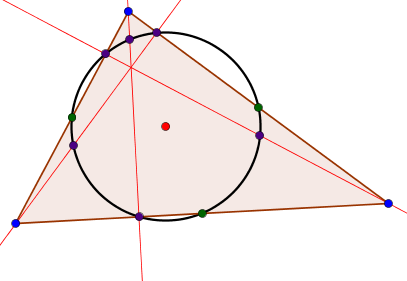
\includegraphics{NPC}
\end{marginfigure}

\setcounter{section}{14}
\section{More Content}

The following are some challenging tasks having to do with the theory of equal content.
The first two are important to us.
The rest are opportunities to show off.

\begin{problem}\label{prob:subtract-rect}
Given two rectangles, $P$ and $R$, construct a square $S$ so that, when taken together the content of $R$ and $S$ is equal to the content of $P$.
\end{problem}

\begin{problem} \label{conj:parallel-in-triangle} Use the theory of content to give a new proof of the midline theorem, Theorem 3.6.
\end{problem}

\begin{challenge}\label{chal:circle-given-two-points-tangent}
Given a line $\ell$ and given two points $A$ and $B$ not lying on $\ell$, construct a circle passing through $A$ and $B$ and tangent to $\ell$.
\end{challenge}

\begin{challenge}\label{chal:circle-point-two-tangents}
Given two lines $\ell$ and $m$ and a point $P$ not on either line, construct a circle through $P$ and tangent to both $\ell$ and $m$.
\end{challenge}

\begin{conjecture}\label{conj:content-triangle}
Let $ABC$ be a triangle, $DE$ a line parallel to the base $BC$, and $F$ the midpoint of segment $DE$, where $D$ lies on ray $AB$ and $E$ lies on ray $AC$. Let $AF$ meet $BC$ at $G$. Then $G$ is the midpoint of $BC$.
\end{conjecture}


\begin{conjecture}\label{conj:content-circle}
Let $\Gamma$ be a circle with center $O$. Let $A$ be a point outside the circle, and $AB$ and $AC$ tangents to $\Gamma$ from $A$, with $B, C$ lying on $\Gamma$. Let $BC$ meet $OA$ at $D$. Then the rectangle on $OA$ and $OD$ has equal content with the square on $OB$.
\end{conjecture}

\begin{conjecture}\label{conj:right-triangle-similarity}
Let $ABC$ be a right triangle with right angle at $A$. Let $AD$ be the altitude from $A$ to side $BC$. The square on side $AD$ has equal content with the rectangle on $BD$ and $DC$.
\end{conjecture}

\begin{conjecture}\label{conj:divide-triangle}
Let $ABC$ be a triangle and $D$ a point on side $BC$. Let $E$ be the midpoint of $BC$ and draw the parallel to $AD$ through $E$. Let this new line meet the union of $AB$ and $AC$ at a point $F$. Then the segment $DF$ cuts the triangle into two polygons of equal content.
\end{conjecture}


\vfill
\end{document}
